%----------------------------------------------------------------
%
%  File    :  thesis-style.tex
%
%  Author  :  Keith Andrews, IICM, TU Graz, Austria
%
%  Created :  27 May 93
%
%  Changed :  19 Feb 2004
%
% styling and technical implementation adopted 2011 by Karl Voit
%----------------------------------------------------------------

					\section{Mathematische Grundlagen}
					\label{chap:Style}

					\subsection{Koordinatensysteme}

					Häufig sind wir daran interessiert, geometrische Dinge in der Mathematik darzustellen um mit ihnen zu rechnen.
					\important{Karthsische Koordinaten} {}
					\beginip
					\begin{center}

					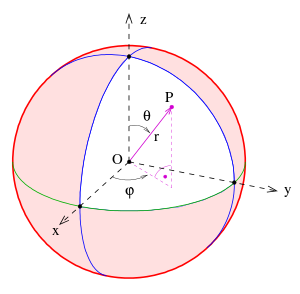
\includegraphics[scale = 0.5	]{kugelkoord.png}

				\end{center}
					\iend

					\formulaBegin
						$\vec{F}(r, \theta, \varphi) = \left(\begin{array}{c} 1 \\ 0 \\ 0 \end{array}\right)_{Kugel\ Koordinaten} = 1 \cdot \vec{e}_r$ \\

					\formulaEnd
					\begin{center}

					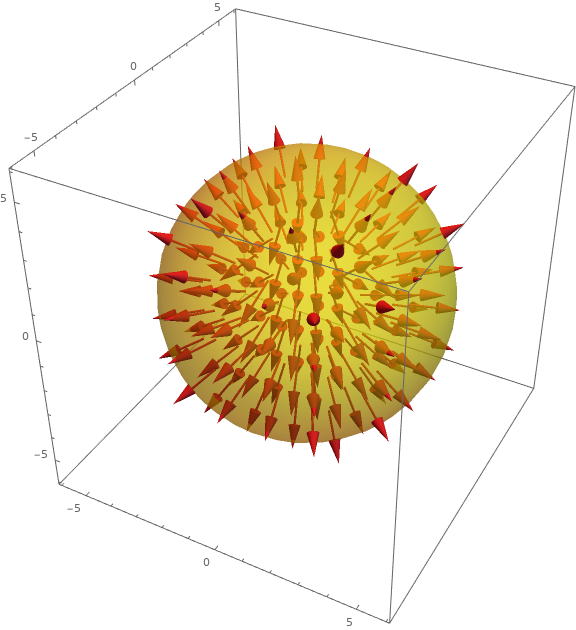
\includegraphics[scale=0.4]{spherical_r.png}

					\end{center}


					\formulaBegin
						$\vec{F}(r, \theta, \varphi) = \left(\begin{array}{c} 0 \\ 1 \\ 0 \end{array}\right)_{Kugel\ Koordinaten} = 1 \cdot \vec{e}_\theta$ \\

					\formulaEnd
					\begin{center}

					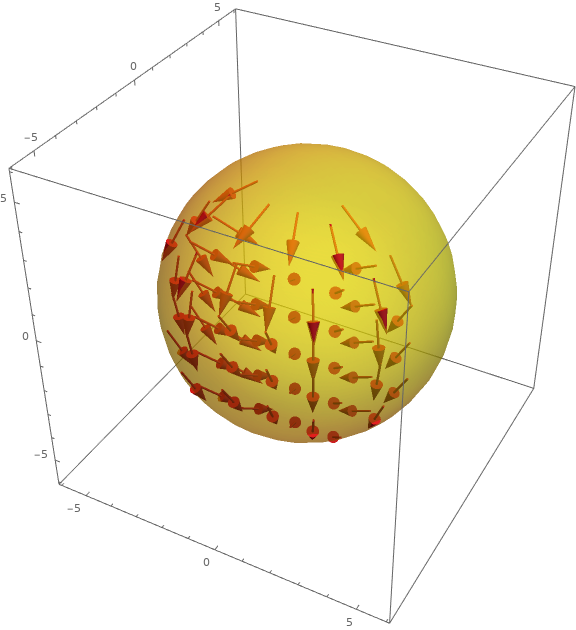
\includegraphics[scale=0.4]{spherical_theta.png}

					\end{center}


					\formulaBegin
						$\vec{F}(r, \theta, \varphi) = \left(\begin{array}{c} 0 \\ 0 \\ 1 \end{array}\right)_{Kugel\ Koordinaten} = 1 \cdot \vec{e}_\varphi$ \\

					\formulaEnd
					\begin{center}

					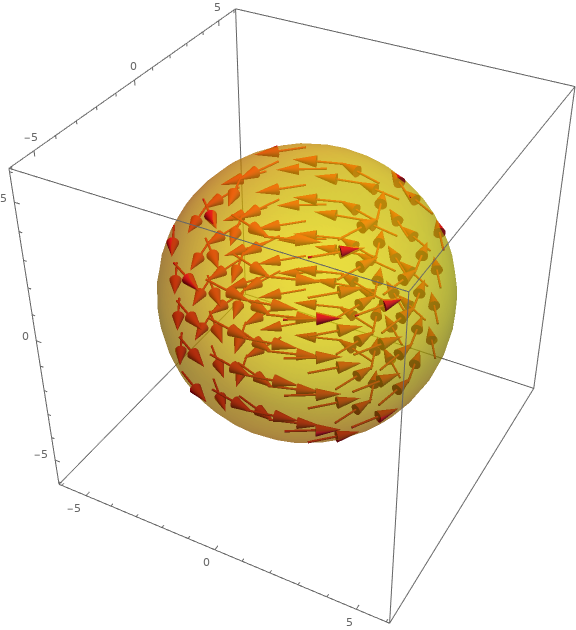
\includegraphics[scale=0.4]{spherical_phi.png}

					\end{center}









					\formulaBegin
						$\vec{F}(\rho, \varphi, z) = \left(\begin{array}{c} 1 \\ 0 \\ 0 \end{array}\right)_{Zylinder\ Koordinaten} = 1 \cdot \vec{e}_\rho$ \\

					\formulaEnd
					\begin{center}

					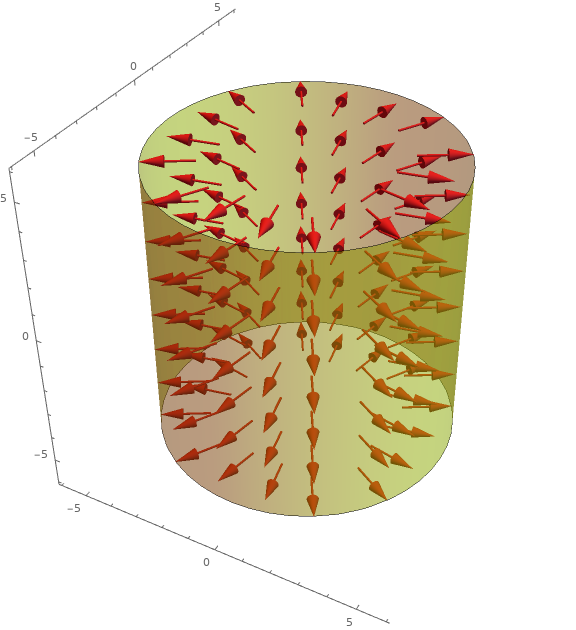
\includegraphics[scale=0.4]{zylindric_rho.png}

					\end{center}


					\formulaBegin
						$\vec{F}(\rho, \varphi, z) = \left(\begin{array}{c} 0 \\ 1 \\ 0 \end{array}\right)_{Zylinder\ Koordinaten} = 1 \cdot \vec{e}_\varphi$ \\

					\formulaEnd
					\begin{center}

					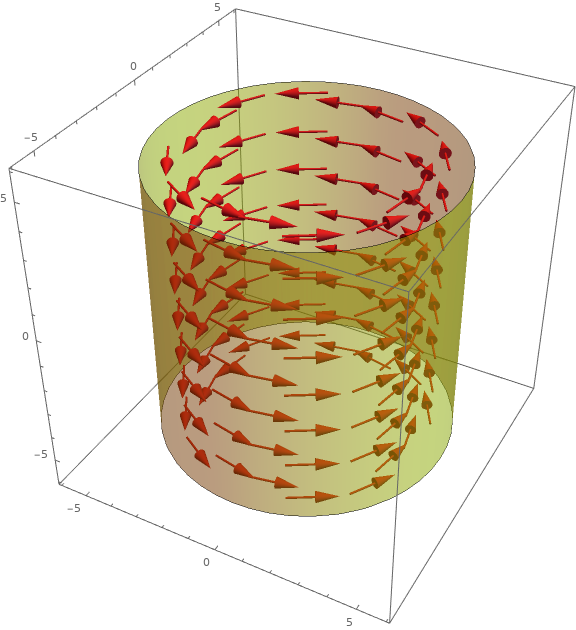
\includegraphics[scale=0.4]{zylindric_phi.png}

					\end{center}




					\formulaBegin
					$\vec{F}(\rho, \varphi, z) = \left(\begin{array}{c} 0 \\ 0 \\ 1 \end{array}\right)_{Zylinder\ Koordinaten} = 1 \cdot \vec{e}_z$ \\

					\formulaEnd
					\begin{center}

					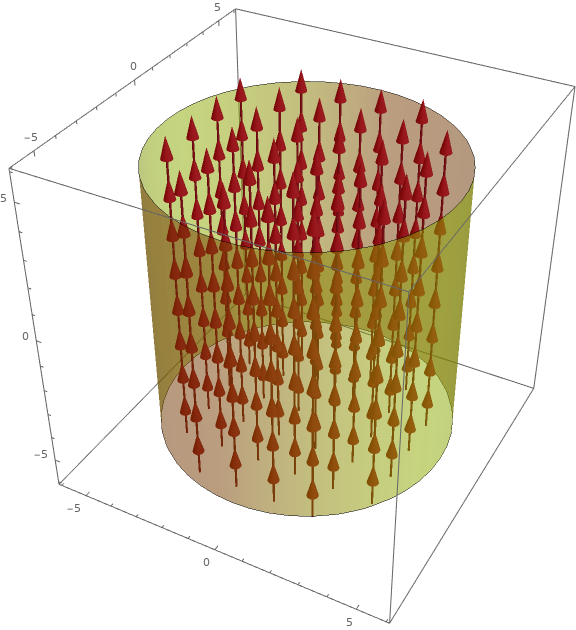
\includegraphics[scale=0.4]{zylindric_z.png}

					\end{center}



					\important{Zylinderkoordinaten} {}
					\beginip

					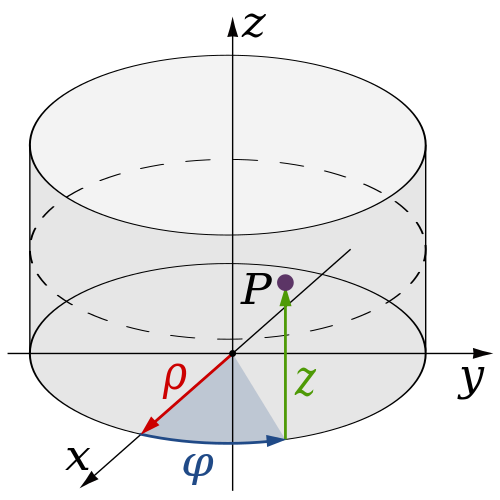
\includegraphics[scale = 0.4]{zylinderkoord.png}
					\iend

					\important{Kugelkoordinaten} {}
					\beginip
					\iend




					\important{Defintion}{Vektorfeld}
					\beginip
						Ein Vektorfeld, bezeichnet eine mathematische Funktion, welche anstatt einer skalaren Grösse, Vektoren zurück gibt. \\
						Häufig ist ein Vektorfeld nicht nur von einer Variable (x) abhängig, sondern besitzt 3 Parameter (x,y,z) die wir manchmal als Ortsvektor $\vec{r}$ zusammenfassen.
					\iend


					\important{Defintion}{Wegintegral über ein Vektorfeld}
					\beginip
					% TODO %

					\iend


					\important{Defintion}{Fluss eines Vektorfeldes}
					\beginip
							\formulaBegin
							$ \oiint_A \vec{E} \cdot d\vec{A}$
							\formulaEnd
							Bezeichnen wir als Oberflächenintegral des Vektorfeldes $\vec{E}$.  Der Wert des Integrales gibt uns eine Information darüber, wieviel Feld durch eine gegebene Hüllfäche "fliesst"

					\iend

					\important{Beispiel}{}
					\beginip
					Wir betrachten ein Rohr der Länge L und mit radius R. \\
					In der Mitte des Rohres im Uhrsprung des Koordinatensystems befindet sich eine Wasserquelle, welche eine gewisse Menge Wasser generiert. \\
					Die Flussdichte des Wassers, ist durch Folgendes Vektorfeld gegeben: \\
					\begin{center}

					$  \vec{J}_{wasser}(x,y,z) = \left\{
					       \begin{array}{@{}l@{\thinspace}l}
					          1 \cdot \vec{e}_y  \cdot [\frac{L}{s \cdot m^2}] &: \frac{-l}{2} < y < \frac{l}{2}\ und\ (x^2 + z^2) \leq R \\
					          0 \cdot \vec{e}_y  \cdot [\frac{L}{s \cdot m^2}] &: sonst\\
					       \end{array}
					       \right$
	 					\end{center}

						\begin{enumerate}
							\item  Zeichne das Vektorfeld in einem 3-Dimensionalen Koordinatensystem. \\
							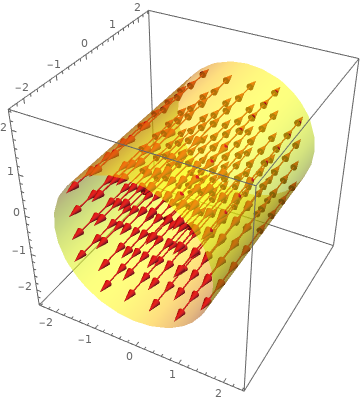
\includegraphics[scale=0.4]{plot.png}
							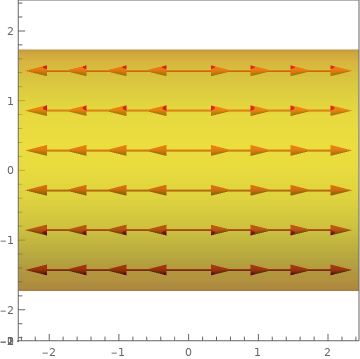
\includegraphics[scale=0.4]{plot2.png}
							\item
						\end{enumerate}
					\iend
